\documentclass[a4paper,12pt]{article} % добавить leqno в [] для нумерации слева
\usepackage[a4paper,top=1.3cm,bottom=2cm,left=1.5cm,right=1.5cm,marginparwidth=0.75cm]{geometry}
%%% Работа с русским языком
\usepackage{cmap}					% поиск в PDF
\usepackage[warn]{mathtext} 		% русские буквы в фомулах
\usepackage[T2A]{fontenc}			% кодировка
\usepackage[utf8]{inputenc}			% кодировка исходного текста
\usepackage[english,russian]{babel}	% локализация и переносы
\usepackage{physics}
\usepackage{multirow}
\usepackage{bm}
\usepackage{longtable}
\usepackage{xcolor}
%%% Нормальное размещение таблиц (писать [H] в окружении таблицы)
\usepackage{float}
\restylefloat{table}


\documentclass[a4paper,12pt]{article}
\usepackage[utf8]{inputenc}
\usepackage[russian]{babel}
\usepackage{amsmath}
\usepackage{amssymb}
\usepackage{graphicx}
\usepackage{geometry}
\usepackage{booktabs}
\usepackage{caption}
\usepackage{enumitem}
\usepackage{siunitx}

\geometry{left=2cm,right=1.5cm,top=2cm,bottom=2cm}
\setlist[enumerate]{label=\arabic*., leftmargin=*}


\usepackage{graphicx}

\usepackage{wrapfig}
\usepackage{tabularx}

\usepackage{hyperref}
\usepackage[rgb]{xcolor}
\hypersetup{
	colorlinks=true,urlcolor=blue
}
\usepackage{pgfplots}
\pgfplotsset{compat=1.9}
%%% Дополнительная работа с математикой
\usepackage{amsmath,amsfonts,amssymb,amsthm,mathtools} % AMS
\usepackage{icomma} % "Умная" запятая: $0,2$ --- число, $0, 2$ --- перечисление

%% Номера формул
%\mathtoolsset{showonlyrefs=true} % Показывать номера только у тех формул, на которые есть \eqref{} в тексте,

%% Шрифты
\usepackage{euscript}	 % Шрифт Евклид
\usepackage{mathrsfs} % Красивый матшрифт

\begin{document}

\section{Формальный отчет}
\begin{enumerate}
    \item Выполнил: Комиссаров Данил Андреевич.
    \item Студент группы Б01-304.
    \item Выполненная схема - Полный сумматор (Full Adder) двух 3-битных входов.
    \item Контакты: komissarov.da@phystech.edu
    \item Полный сумматор — логическая схема, которая производит сложение двух трехбитных чисел и одного однобитного числа, обозначаемых A(а0 - младший бит, а1 - средний бит, а2 - старший бит), Б(б0 - младший бит, б1 - средний бит, б2 - старший бит) и входной бит переноса. На выход подаются трехбитное число В(в0 - младший бит, в1 - средний бит, в2 - старший бит) и выходной бит переноса., где В — это сумма по модулю 8 (а в общем случае $2^n$), а выходной бит переноса - это флаг, который говорит о переполнении выхода.
    \item 
    \begin{figure}[H]
        \centering
        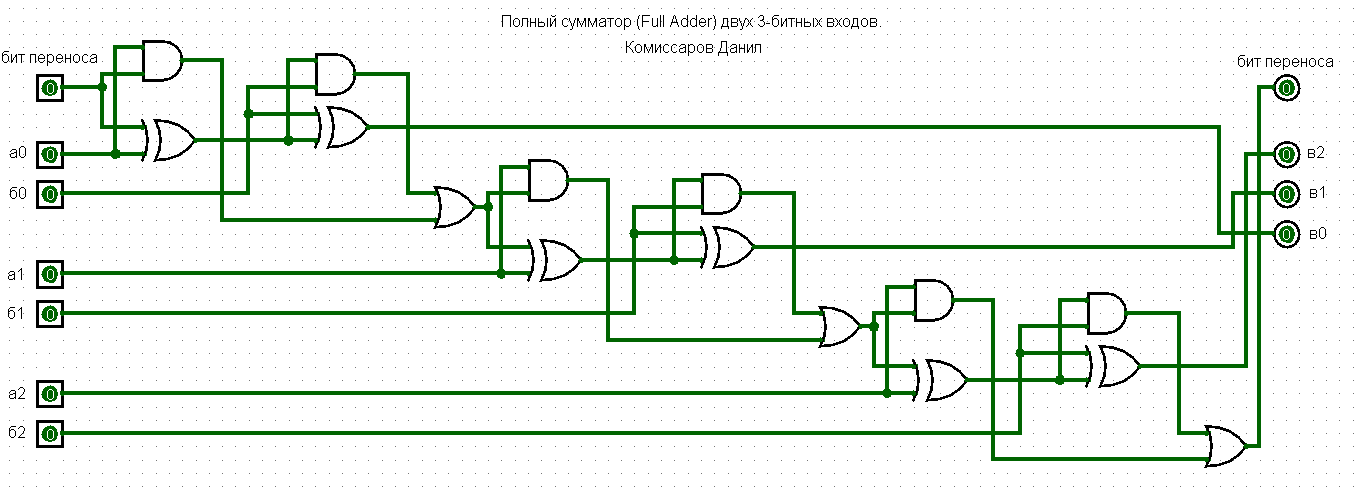
\includegraphics[width=1\linewidth]{Formal/Photo1.png}
    \end{figure}
    \begin{figure}[H]
        \centering
        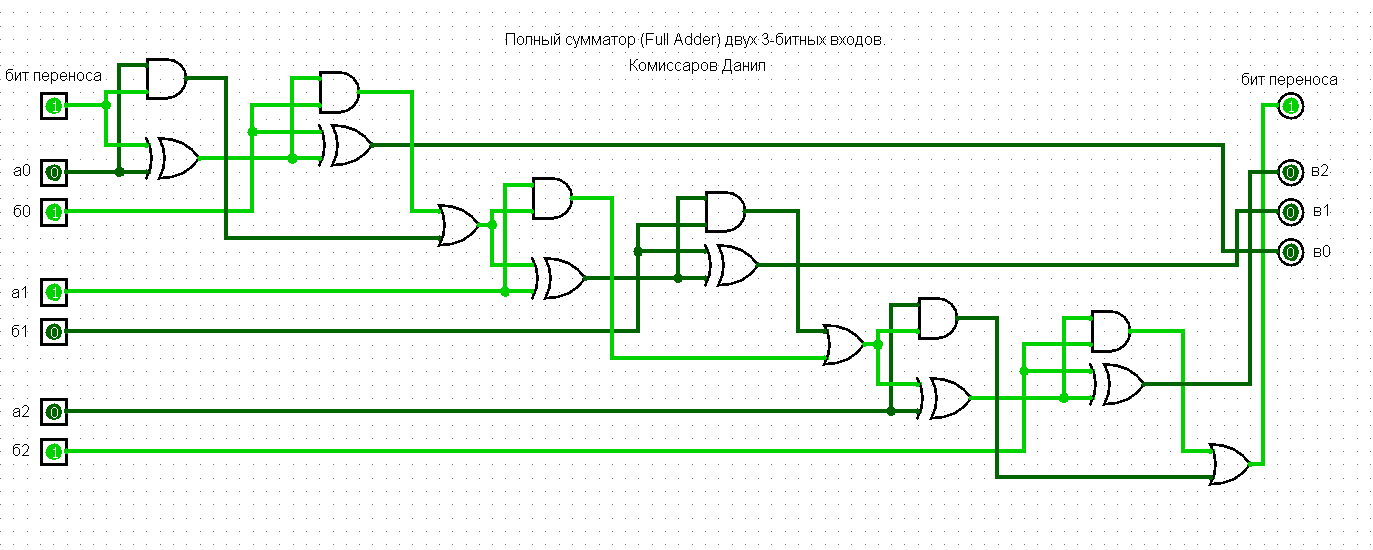
\includegraphics[width=1\linewidth]{Formal/Photo2.png}
    \end{figure}
    \begin{figure}[H]
        \centering
        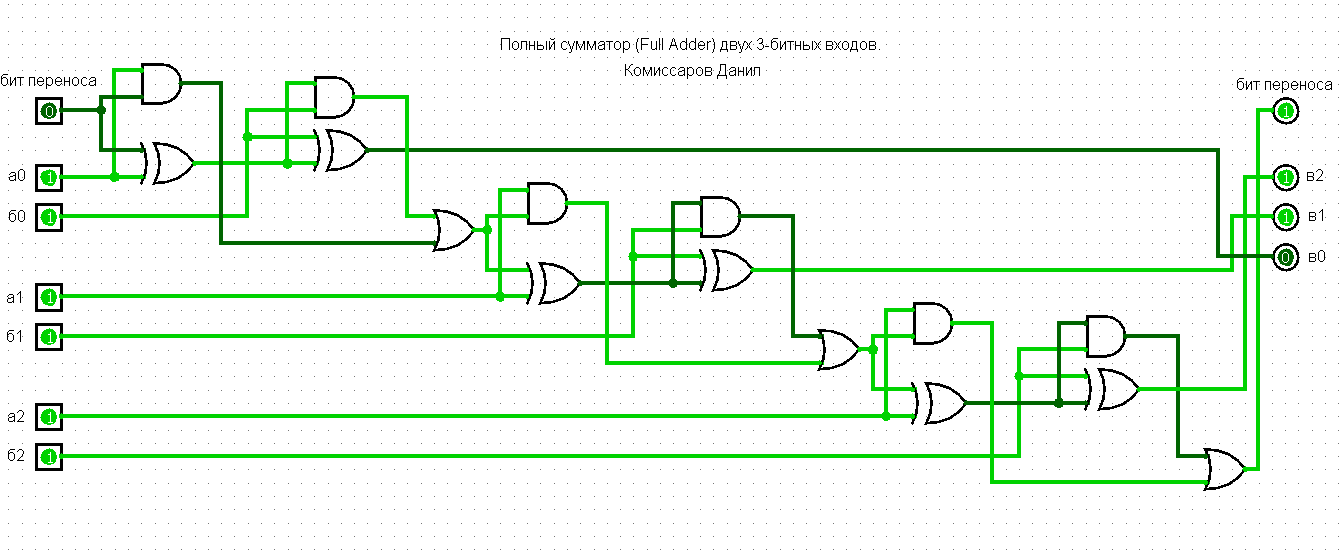
\includegraphics[width=1\linewidth]{Formal/Photo3.png}
    \end{figure}
    \begin{figure}[H]
        \centering
        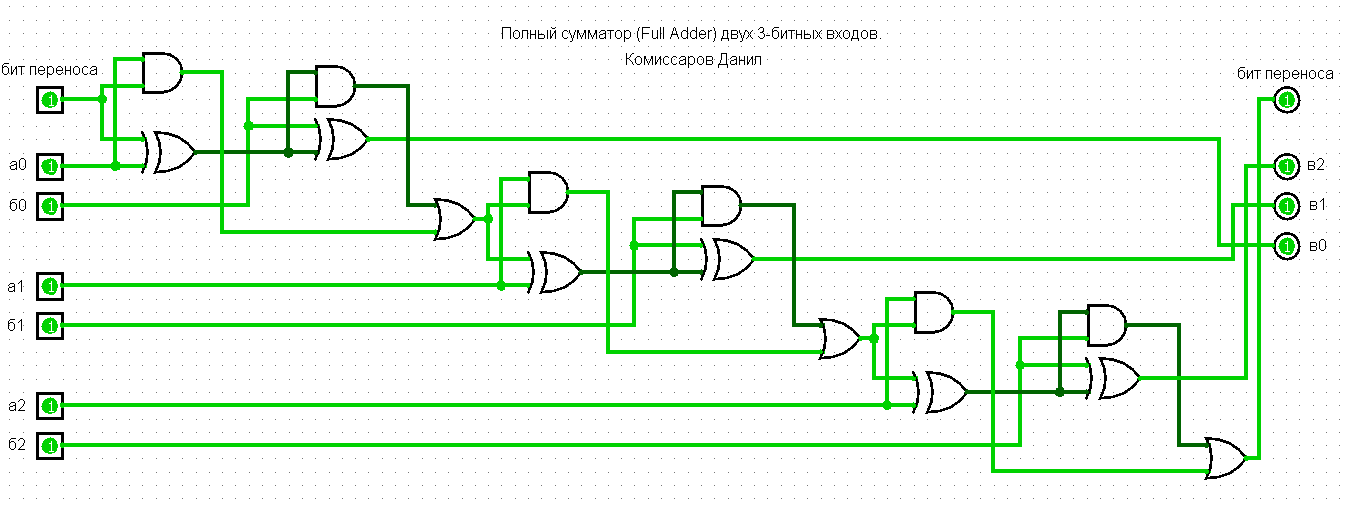
\includegraphics[width=1\linewidth]{Formal/Photo4.png}
    \end{figure}
    \item Критическое время составляет 9t
    \begin{figure}[H]
        \centering
        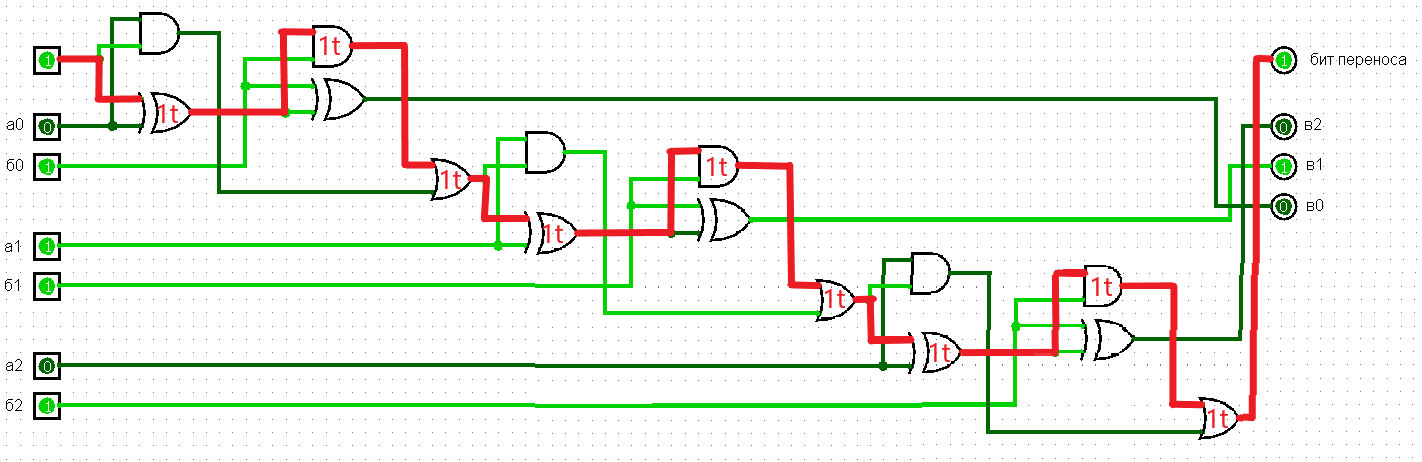
\includegraphics[width=1\linewidth]{Formal/Crit way.png}
    \end{figure}
    \item Схема состоит из 60-ти полевых транзисторов.
\end{enumerate}

\end{document}